\chapter{Introduction}
\label{intro}

\section{Reconfigurable Architectures}
Recent trends in technology scaling, the availability of large amounts of data,
and novel algorithmic breakthroughs have spurred accelerator architecture
research. Reconfigurable architectures like field-programmable gate arrays
(FPGAs) and coarse-grain reconfigurable architectures (CGRAs) have received
renewed interest from academic researchers and industry practitioners alike,
primarily due to their potential performance and energy efficiency benefits over
conventional CPUs. For instance, FPGAs are now being used to accelerate web search
in datacenters at Microsoft and Baidu~\cite{catapult, baidu},
Amazon now offers FPGA instances as part of AWS~\cite{awsf1},
and Intel has announced products like in-package Xeon-FPGA systems~\cite{harp}
and FPGA-accelerated storage systems~\cite{nand_flash}.
Similarly, several recent research prototypes~\cite{dyser, ti, scaledeep, scnn, plasticine}
and startups~\cite{wavecomp, nervana} have explored various
kinds of CGRAs at different granularities, with the number of startups in this
area seemingly growing by the day.
Growing use of such reconfigurable architectures has made them more available
to programmers now than ever before.

Reconfigurable devices are able to accelerate applications, in part, by exploiting multiple
levels of nested parallelism and data locality with custom data pipelines and memory hierarchies.
Unfortunately, the same features that make reconfigurable architectures efficient
also make them much more complex to program. In FPGAs, an accelerator design
must account for the timing between pipelined signals and the physically limited
compute and memory resources available on the target device.
It must also manage partitioning of data between local scratchpads and off-chip memory to achieve good data locality and effective memory bandwidth.
The combination of these complexities can easily lead to intractable accelerator design spaces, even for relatively small applications~\cite{cascaval}.

These challenges have caused programmability to be a key limiting factor to widespread adoption and FPGAs~\cite{fpgaMasses,DeSutter2013}.
%The space of CGRA programmability is currently fragmented with incompatible, architecture-specific programming models.
The state of the art in programming FPGAs involves using a combination of vendor-supplied IP blocks,
hand-tuned hardware modules written using either low-level RTL or high-level synthesis tools,
and architecture-specific glue logic to communicate with off-chip components such as DRAM.
Hardware description languages (HDLs) like Verilog and VHDL are designed for explicit specification of hardware,
placing the burden on the user to solve essentially all of the complexities of implementing their algorithm in hardware.

\section{High Level Synthesis}
Commerical high-level synthesis (HLS) tools like SDAccel~\cite{sdaccel}, Vivado HLS~\cite{vivadohls},
and Intel's OpenCL SDK~\cite{opencl_sdk} raise the level of abstraction compared to HDLs significantly.
For example, HLS tools allow programmers to write accelerator designs in terms of untimed, nested loops
and offer library functions for common operations like data transfer between a CPU host and the FPGA.
However, existing commercial HLS tools have all been built on top of software languages like C and OpenCL.
These software languages were originally designed to target instruction-based processors with a cached, uniformly addressable memory space.
This is clearly apparent in each language's semantics and memory model.
For example, the concept of pointers in C and C++ essentially assume a memory system which is flat, one dimensional, and uniformly accessible.
Describing the nuances of accessing memory in a more complicated system, such as the combination of main memory and
scratchpads on an FPGA inherently requires additional information to be easily expressible in the language.
In practice though, this additional information is supported in HLS tools through language
extensions in the form of optional user pragmas.

Consequently, although existing HLS tools raise the level of abstraction for targeting reconfigurable architectures,
they do so with an ad-hoc, often underspecified mix of software and hardware abstractions.
This, in turn, results in difficulties in HLS compiler implementations.
For instance, while SDAccel can convert nested loops into hardware state machines,
the language's compiler does not allow pipelining of loops at arbitrary nesting levels~\cite{vivado_userguide}.

When using high level synthesis tools, programmers must keep in mind that,
despite the software programming abstractions, they must employ hardware,
not software, optimization techniques when using HLS tools~\cite{nane2016survey}.
Additionally, compile times for HLS can often be long for large designs due to
complications that arise during pipeline scheduling~\cite{Aladdin}.
Such limitations restrict the user's ability to explore more complex design spaces.
For most domain experts, this makes it challenging to write code which produces fully optimized designs.

\section{Domain-Specific Languages}
% Based on recent trends in machine learning and and data analytics, high level
% domain-specific languages (DSLs) like Pytorch~\cite{pytorch} and TensorFlow~\cite{tensorflow} may be
% the ideal programming model for many domain experts.
% These languages have little or no target hardware information at all, but
% instead providing a high level environment for users to productively explore
% program designs within their domain. Fortunately, such a high level of abstraction
% may also make these languages prime candidates for compiling to FPGAs.
As demands for specialization in hardware have been growing, so too have the demands for
specialization in software programming models for improved CPU and GPU performance and programmer productivity.
DSLs help to serve this goal by presenting the user with a very high level of abstraction, generally
at the cost of a reduced number of possible operations and data structure types.
This focus in turn allows domain-specific types and operations to be isolated as
higher level operators with semantic information which the compiler is aware of,
enabling optimizations that would otherwise be difficult or impossible.
The use of DSLs has become particularly prominent lately in the field of machine learning (ML),
where new models and ideas are being tried ever more rapidly. Pytorch~\cite{pytorch} and TensorFlow~\cite{tensorflow}, for example,
provide high levels of abstraction for building machine learning models for inference and training.

The key benefit of domain-specific languages lie in this
high level of abstraction, which is typically almost entirely removed from any target
architecture. This level of abstraction makes DSLs a very promising choice for targeting FPGAs.
It also gives the DSL compiler a great deal of freedom in what it can do to implement the
desired operations. Unfortunately, this degree of freedom also implies huge design spaces
which can be challenging to navigate.
In existing DSL compilers that target reconfigurable hardware (usually FPGAs),
these complexities are solved using a kernel-based approach.
The DSL compiler performs domain-specific operations, then lowers the resulting
abstraction directly to a hardware implementation using either pre-existing, hand-written kernels in
an HDL or implementations written in a high level synthesis language~\cite{george14fpl}.
In these kernel-wise techniques, the compilation path tends to miss key cross-operation optimizations
like fusion and tiling, resulting in excessive transfers to and from main memory.

\section{A Framework for DSLs to FPGAs}
The key problem with existing DSL FPGA backends is that they attempt
to bridge two vastly different levels of abstraction with no intermediate
levels. This restricts the types of optimizations the compiler can reasonably
perform, and consequently leads to inefficient designs.
In this work, we propose a practical framework using this
new compiler for automatic generation of
efficient accelerators implemented on reconfigurable architectures starting
from domain-specific languages. As shown in Figure~\ref{fig:system-diag}, this
framework improves upon existing approaches by introducing two intermediate levels of
abstraction where key optimizations and tradeoff decisions can be made.

\begin{figure*}
\centering
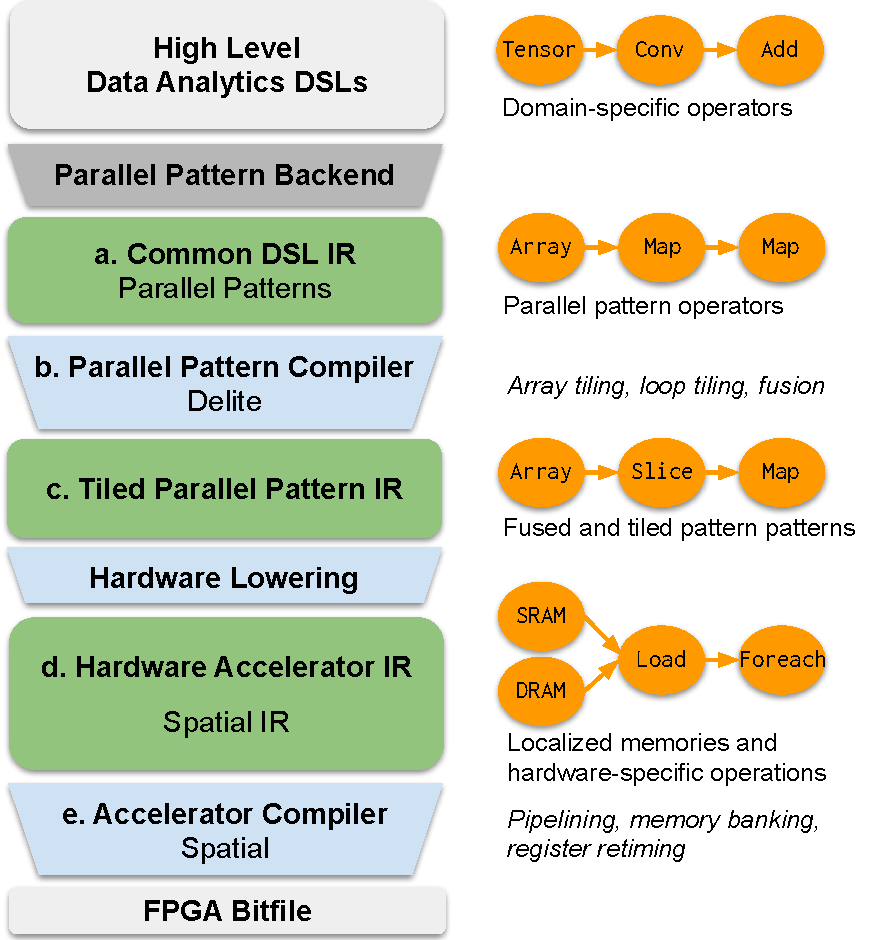
\includegraphics[height=12cm]{1-intro/figs/system-diag}
\caption{\label{fig:system-diag}Block diagram of the compiler framework proposed in this work.
The framework compiles high level domain specific languages (DSLs) from a
common parallel pattern intermediate representation (IR). Using a compiler
called Delite, this IR is optimized, transformed, and lowered to a lower level
intermediate representation for hardware accelerator designs called the Spatial IR.
This lower level IR is compiled by the Spatial compiler and generated
as an efficient hardware accelertaor design for a selected FPGA target.}
\end{figure*}

The system first presents DSL compilers with a common intermediate abstraction composed of
parallel patterns like \emph{Map}, \emph{Reduce}, and \emph{FlatMap} (Figure~\ref{fig:system-diag}a.).
A DSL targeting our framework lowers its operations to implementations using these patterns.
We chose these abstractions because, in previous work, parallel patterns have
been shown to serve the dual purpose of raising the
level of abstraction for the
programmer~\cite{ecoop13sujeeth,pldi13halide}, and providing richer
semantic information to the compiler about data parallelism
and access pattern information~\cite{delite-tecs14}.
Specifically, we build on the existing body of work
on the Delite compiler, which has previously been shown
to provide a good, common set of parallel patterns across many computation domains in data analytics, including
image processing, database processing, and machine learning~\cite{pldi13halide,ecoop13sujeeth}.

Compilation in the framework is composed of two phases. In the first phase,
a high level compiler performs optimizations like loop fusion and tiling
on the parallel pattern IR (Figure~\ref{fig:system-diag}b.), resulting in an
optimized, tiled parallel pattern IR (Figure~\ref{fig:system-diag}c.).

The portion of the IR targeted for hardware acceleration is then automatically
lowered into a novel, hardware-specific intermediate
representation (Figure~\ref{fig:system-diag}d.).
We introduce this new representation, which we call the Spatial IR,
in this work to address the problems in existing
high-level synthesis tools. In particular, we identify several key
abstractions required to create a new high-level synthesis language from the
ground up and use these abstractions to build an intermediate representation
specific for creating hardware accelerator designs for FPGAs.
We suggest that this ``clean slate'' approach to high-level synthesis abstraction
design leads to a representation which is semantically cleaner when targeting
reconfigurable architectures, particularly when optimizing for data locality and parallelism.
These abstractions help the compiler to more easily optimize designs for improved performance.

The Spatial IR is then optimized and lowered further by the hardware accelerator design compiler (Figure~\ref{fig:system-diag}e.), referred to hereafter as the Spatial compiler.
In this work, we describe the Spatial compiler and several key optimizations it
performs for produces performant hardware accelerator designs.
These optimizations include specialization of on-chip memories based on access patterns and
automatic pipelining of arbitrarily nested loops.
We also discuss an optional automated search of the hardware design space
to analyze tradeoffs and improve design performance.
We describe two approaches to this automated search, one using basic heuristic random
search and a faster approach using an active machine learning framework called
HyperMapper~\cite{Bodin2016:PACT16} to drive exploration.

When targeting FPGAs, we show that Spatial generates optimized, synthesizable
code along with C++ code which can be used on a host CPU to administrate
initialization and execution of the accelerator on the target FPGA.
Spatial currently supports Xilinx Ultrascale+ VU9P FPGAs on Amazon's
EC2 F1 Instances, Xilinx Zynq-7000 and Ultrascale+ ZCU102 SoCs, and Altera DE1 and Arria 10 SoCs.
While the constructs in Spatial are general across reconfigurable architectures
and can also be used to target CGRAs, in this work we focus on Spatial in the
context of our larger framework targeting FPGAs.

\section{Contributions}
The system proposed in this work was developed on the shoulders of work done by
the Delite team within the Pervasive Parallelism Lab at Stanford University.
While the Spatial compiler is a novel implementation begun with this work, it
is inspired heavily by prior Delite and DSL compiler work.
The core of Spatial's IR and compiler,
dubbed ``Argon'', began as a customized rewrite of Lightweight Modular Staging (LMS)
by Tiark Rompf, et. al.~\cite{tiark-thesis,lms} with additional considerations for managing
compiler metadata improving compiler performance.
Further discussion of the design decisions around the Argon framework with respect
to the implementation of the Spatial language and compiler can be found in Appendix~\ref{argon}.
Hassan Chafi~\cite{hassan-thesis} and
Arvind Sujeeth~\cite{arvind-thesis} showed the expressitivity benefits of
parallel-pattern based DSLs across a wide variety of domains.
Kevin Brown~\cite{kevin-thesis}
showed the performance benefits of parallel pattern
could be extended across multi-core and cluster CPUs, while
HyoukJoong Lee showed that the same approach can be used to target GPUs
and FPGAs~\cite{hj-thesis}. While the focus of this work is on targeting FPGAs,
we briefly show in Chapter~\ref{plasticine-evaluation} that this approach
can be generalized to coarse-grained reconfigurable architectures (CGRAs) as well.

The key contribution of this work is the proposal and demonstration of a system
which generates efficient, performant hardware accelerator designs
for FPGAs from high level, domain specific languages.
We further summarize the core contributions of this work are as follows:
\vspace{-5pt}
\begin{itemize}
  \item We describe a systematic set of rules for tiling parallel patterns.
  Unlike previous automatic tiling work, these rules are based on pattern matching
  and therefore do not restrict all memory accesses within the program to be affine.

  \vspace{5pt}

  \item We present experimental results for a set of benchmark applications
  from the data analytics domain running on an FPGA and show the performance impact of
  the described high level transformations.

  \vspace{5pt}

  \item We discuss the abstractions required to describe target-agnostic accelerator designs for FPGAs.
  We then describe our novel implementation of these constructs in the Spatial intermediate representation.

  \vspace{5pt}

  \item We demonstrate a method for automatically lowering a parallel pattern IR
  to hardware structures. We also show how to automatically generate coarse-grained pipelines, a
  generalization of pipelines that greatly increase design throughput.

  \vspace{5pt}

  \item We describe hardware-specific optimizations in the Spatial compiler, including
  pipeline retiming, memory banking, and two methods for automated design parameter tuning.

  \vspace{5pt}

  \item We evaluate the performance of the designs generated by the Spatial compiler
  and the Spatial compiler's design parameter tuning strategies. We also evaluate the generality of the Spatial abstraction ability to efficiently express a wide variety of applications.
  We demonstrate that Spatial is able to achieve better performance than Xilinx's commercial high level synthesis tool, SDAccel, on a diverse set of data analytics benchmarks, with a geometric mean speedup of $2.9\times$.
\end{itemize}

\section{Outline}
Chapter~\ref{background} provides background on domain-specific languages and parallel patterns.
We also formalize the set of parallel patterns we will discuss in this work.
In Chapter~\ref{delite} we discuss the high level transformations and optimizations for compiling
DSLs to a lower level hardware abstraction.
Chapter~\ref{spatial} then discusses our requirements for our improved intermediate hardware abstraction.
We specify the implementation of this abstraction, the Spatial language, and describe the lowering
process from parallel patterns to Spatial.
Chapter~\ref{compiler} then describes Spatial's intermediate representation and compiler, detailing the transformations and hardware-specific optimizations that it performs.
In Chapter~\ref{related}, we discuss related work across the system, including a discussion of
prior work on automated tiling and high level synthesis languages.
We conclude in Chapter~\ref{conclusion} with a summary and discussion of future opportunities for optimization
and generalization in targeting FPGAs from DSLs using the compiler stack approach.
Appendix~\ref{argon} describes the Argon compiler framework
which both the high level and low level compiler are
built on, and highlights the primary improvements over its predecessor and lessons learned during its development.
